 \chapter{结果分析}
 本文的实验均在安装了Windows 10专业版的台式机上完成,
 实验平台环境如表\ref{tab_pc}所示。
 用于采集数据的扫描设备参数如表\ref{tab_kinect}。
 本章的实验主要在三个样例上进行,
 这三个样例分别为giraffe、pillow和tube。
 这三个样例在现实中的样子和重建后模型如图\ref{static_model}所示。
 本章将展示更多本文的实验结果。
 章节\ref{sec_pose_est_res}将展示在不同的物体位姿下位姿估计算法的结果;
 章节\ref{sec_keyframe_res}将展示捕捉形变并提取关键帧的结果;
 章节\ref{sec_subspace_res}将展示形变子空间的相关结果。
\begin{table}[htp]
    \zihao{5}
    \caption{实验平台参数}
    \label{tab_pc} 
    \centering
    \begin{tabular}[t]{|l|l|c|}
        \hline
        \multirow{3}*   {硬件}  &    CPU        &   Intel® Core™ i5-4430 主频3.00GHz,四核四线程\\
        \cline{2-3}
                                &    GPU         &   NVIDIA GeForce GTX 760,显存4GB\\
        \cline{2-3}
                                &    内存        &   16GB\\
        \hline
        \multirow{2}*   {软件}  &    CUDA        &   CUDA 8.0\\
        \cline{2-3}
                                &    Kinect SDK  &   Kinect SDK 1.8\\
        \hline
    \end{tabular}
\end{table}
\begin{table}[htp]
    \zihao{5}
    \caption{扫描设备参数}
    \label{tab_kinect}
    \centering
    \begin{tabular}[t]{|l|c|}
        \hline
        扫描设备        &   Kinect for Xbox 360\\
        \hline
        RGB图像         &   分辨率$640 \times 480$,深度32位\\
        \hline
        深度图像        &   分辨率$640 \times 480$,深度16位\\
        \hline
        传感深度范围    &   1.2m-3.5m\\
        \hline
        % 最大FPS        &    30\\
        % \hline
    \end{tabular}
\end{table}
 \section{初始位姿估计结果}\label{sec_pose_est_res} 
 图\ref{align_result}展示了各样例的对齐结果。
 其中前两列为giraffe在两种不同位姿下的估计结果,
 第三列为pillow的估计结果,
 第四列为tube的估计结果。
 图中每一列为每一种位姿下位姿估计算法的结果;
 第一行为手部点云分割的结果,
 蓝色的像素为分割出的手部点云;
 第二行为物体点云分割的结果,
 红色的像素为分割出的物体点云;
 第三行为根据估计出的位姿将模型渲染到RGB图像的结果;
 第四行为直接将模型平移到物体点云包围盒中心后的结果;
 第五行为模型和物体点云对齐后的得结果模型以估计出的位姿变换。
 从图中可以看出,
 在各种位姿下,
 本文的算法都能准确的分割出点云并将其与模型对齐,
 从而估计出物体的位姿。
 最后的对齐结果中,
 调整位姿后的模型和根据深度图像生成的点云间仍然存在一定的偏移。
 但这样的对齐效果足够作为ICP算法的初值,
 用ICP算法做局部对齐消除偏移。
 在形变捕捉的过程中,
 每一帧都会用ICP算法估计物体的刚体变换,
 所以模型初始位姿中这些偏移不会对后续的算造成影响。
 \begin{figure}
    \centering
    \includegraphics[width = \textwidth]{./Pictures/align_result_muti_model.png}
    \caption{不同位姿下的位姿估计结果}
    \label{align_result}
\end{figure}
\begin{table}
    \zihao{5}
    \caption{物体点云分割数据}
    \label{tab_sample_data} 
    \centering
    \begin{tabular}[t]{|l|c|c|c|}
        \hline
        样例       &   顶点数   &   面片数   &  物体点云顶点数\\
        \hline
        giraffe     &   1551    &   3000    &   10189       \\
        \hline
        pillow      &   3008    &   6000    &   16090       \\
        \hline
        tube        &   5019    &   10000   &   11653       \\
        \hline
    \end{tabular}
\end{table}

表\ref{tab_sample_data}给出了各样例的基本属于以及初始位姿估计时分割出的物体点云的顶点数;
表\ref{tab_est_pose_time}为各样例在初始位姿估计各阶段的耗时。
表\ref{tab_est_pose_time}中将颜色过滤单独划出,
并不算在手部分割中,
是因为该步骤是在讲RGB图向深度图映射时在GPU上实现的,
这样只需要向GPU传输一次颜色数据。
物体点云分割耗时指的是获取手部点云后,
根据手部点云后根据手部位置寻找物体点云的耗时。
从表\ref{tab_est_pose_time}中可以看出,
用于点云分割的三个步骤耗时很小,
最耗时的是点云对齐。
点云对齐的耗时也与模型的大小无关,
因为对齐前会对物体点云和网格模型中的顶点均匀采样。
本文用于对齐的样本大小与分割出的物体点云中顶点的个数成正比,
所以点云对齐的耗时和物体点云的大小正相关。
\begin{table}
    \zihao{5}
    \caption{位姿估计耗时}
    \label{tab_est_pose_time} 
    \centering
    \begin{tabular}[t]{|l|c|c|c|c|c|}
        \hline
        样例        &   颜色过滤耗时   & 手部分割耗时    &   物体点分割耗时    & 点云对齐耗时    &   总耗时\\
        \hline
        giraffe    &    0.0376s       &  0.0087s       &    0.0336s         &   0.3973s     &   0.4773s\\
        \hline
        pillow     &    0.035s        &  0.0067s       &    0.0302s         &   0.7707s     &   0.8427s\\
        \hline
        tube       &    0.0309s       &  0.0109s       &    0.0317s         &   0.437s      &   0.5005s\\             
        \hline
    \end{tabular}
\end{table}
\section{关键帧提取结果}\label{sec_keyframe_res}
在形变捕捉步骤中,
本文捕捉每一帧中物体发生的形变,
算法的FPS在8至12之间。
样例giraffe的形变捕捉的结果已经在图\ref{deformation_sampling_demo}中展示,
样例pillow和tube的形变捕捉结果在图\ref{ds_p_t}中展示。
\begin{figure}
    \centering
    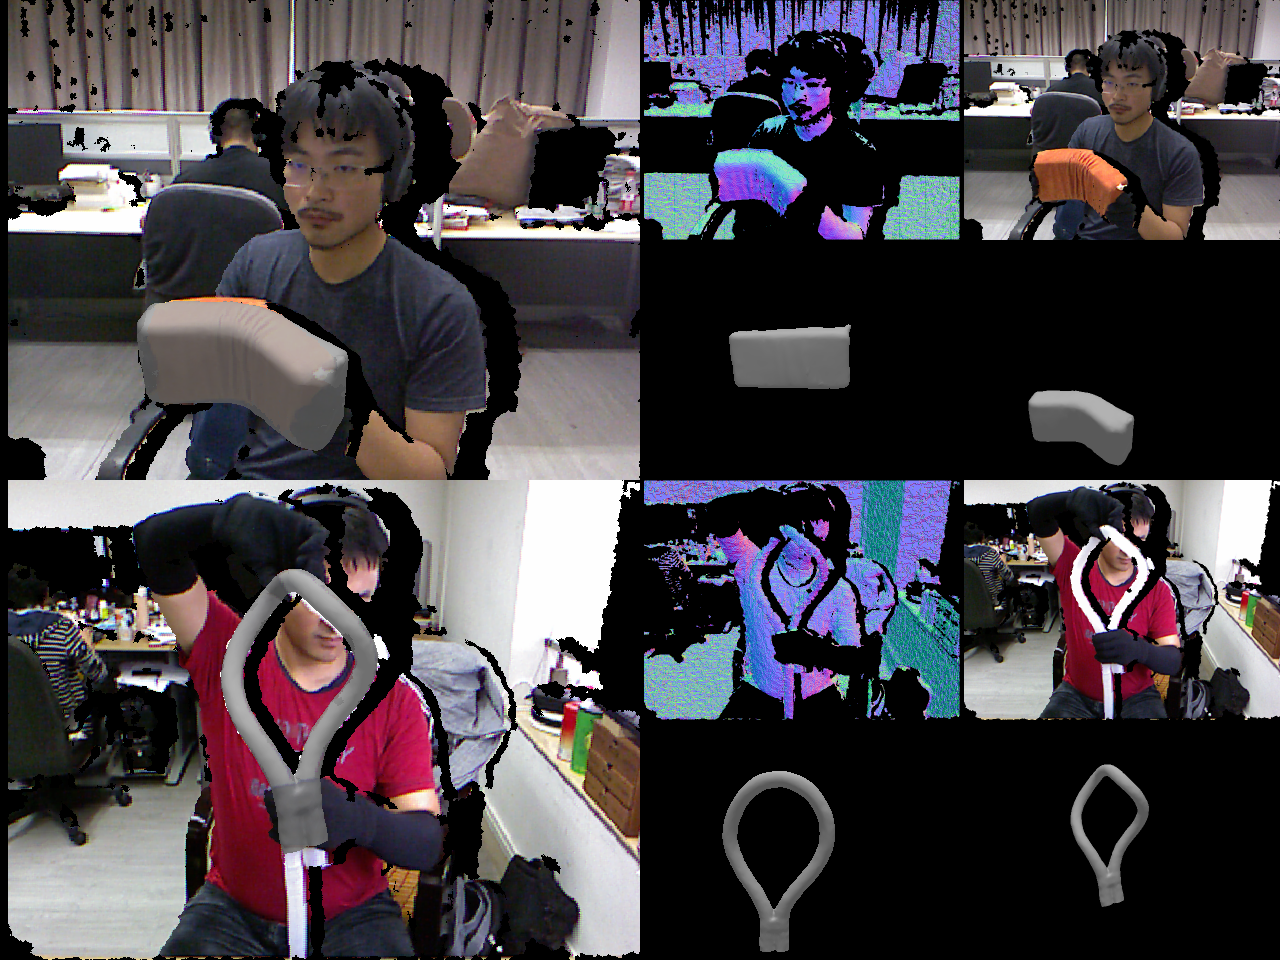
\includegraphics[width = \textwidth]{./Pictures/ds_p_t.png}
    \caption{样例pillow和tube的形变捕捉结果}
    \label{ds_p_t}
\end{figure}

本文采用了通用的形变描述方式,
并不需要形变的物体属于特定的类型,
如人手、人脸等。
因此本文能够捕捉大部分柔性物体的形变。
本文会从捕捉到的形变模型中挑选出部分有代表性的形变状态作为用于构建形变子空间的形变关键帧。
这些关键帧都会根据手部覆盖的区域对齐,消除冗余的刚体变换分量。
样例giraffe的形变关键帧,
以及对齐的结果以及在图\ref{before_after_align}和图\ref{align_area}中展示,
图\ref{pillow_tube_keyframe}展示了样例pillow和tube的形变关键帧和对齐后的结果。
第一行为pillow提取关键帧的结果,
第二行为tube提取关键帧的结果;
每行的第一张为未形变的模型,
最后一张为形变关键帧对齐的结果,
图中红色的部分为模型中用于对齐的部分。
形变捕捉的过程用没有用到特定类型物体的先验知识,
giraffe为长颈鹿形的毛绒玩具,pillow为小枕头,tube为塑料水管,
它们的形变都能很好的被捕捉。
而在对齐之后,本文消除了关键帧中整体偏移,
保证了由此构建出的形变子空间更加准确。

在之前的基于样例形变方法中,
样例都是人工编辑而成,耗费人力和时间。
而且对于现实中存在的物体,
人工编辑的形变样例也不一定满足物体本身的形变特性。
本文的所有形变关键帧全部通过捕捉物体在现实世界中的形变得到,
保证了形变关键帧的准确性。
\begin{figure}
    \centering
    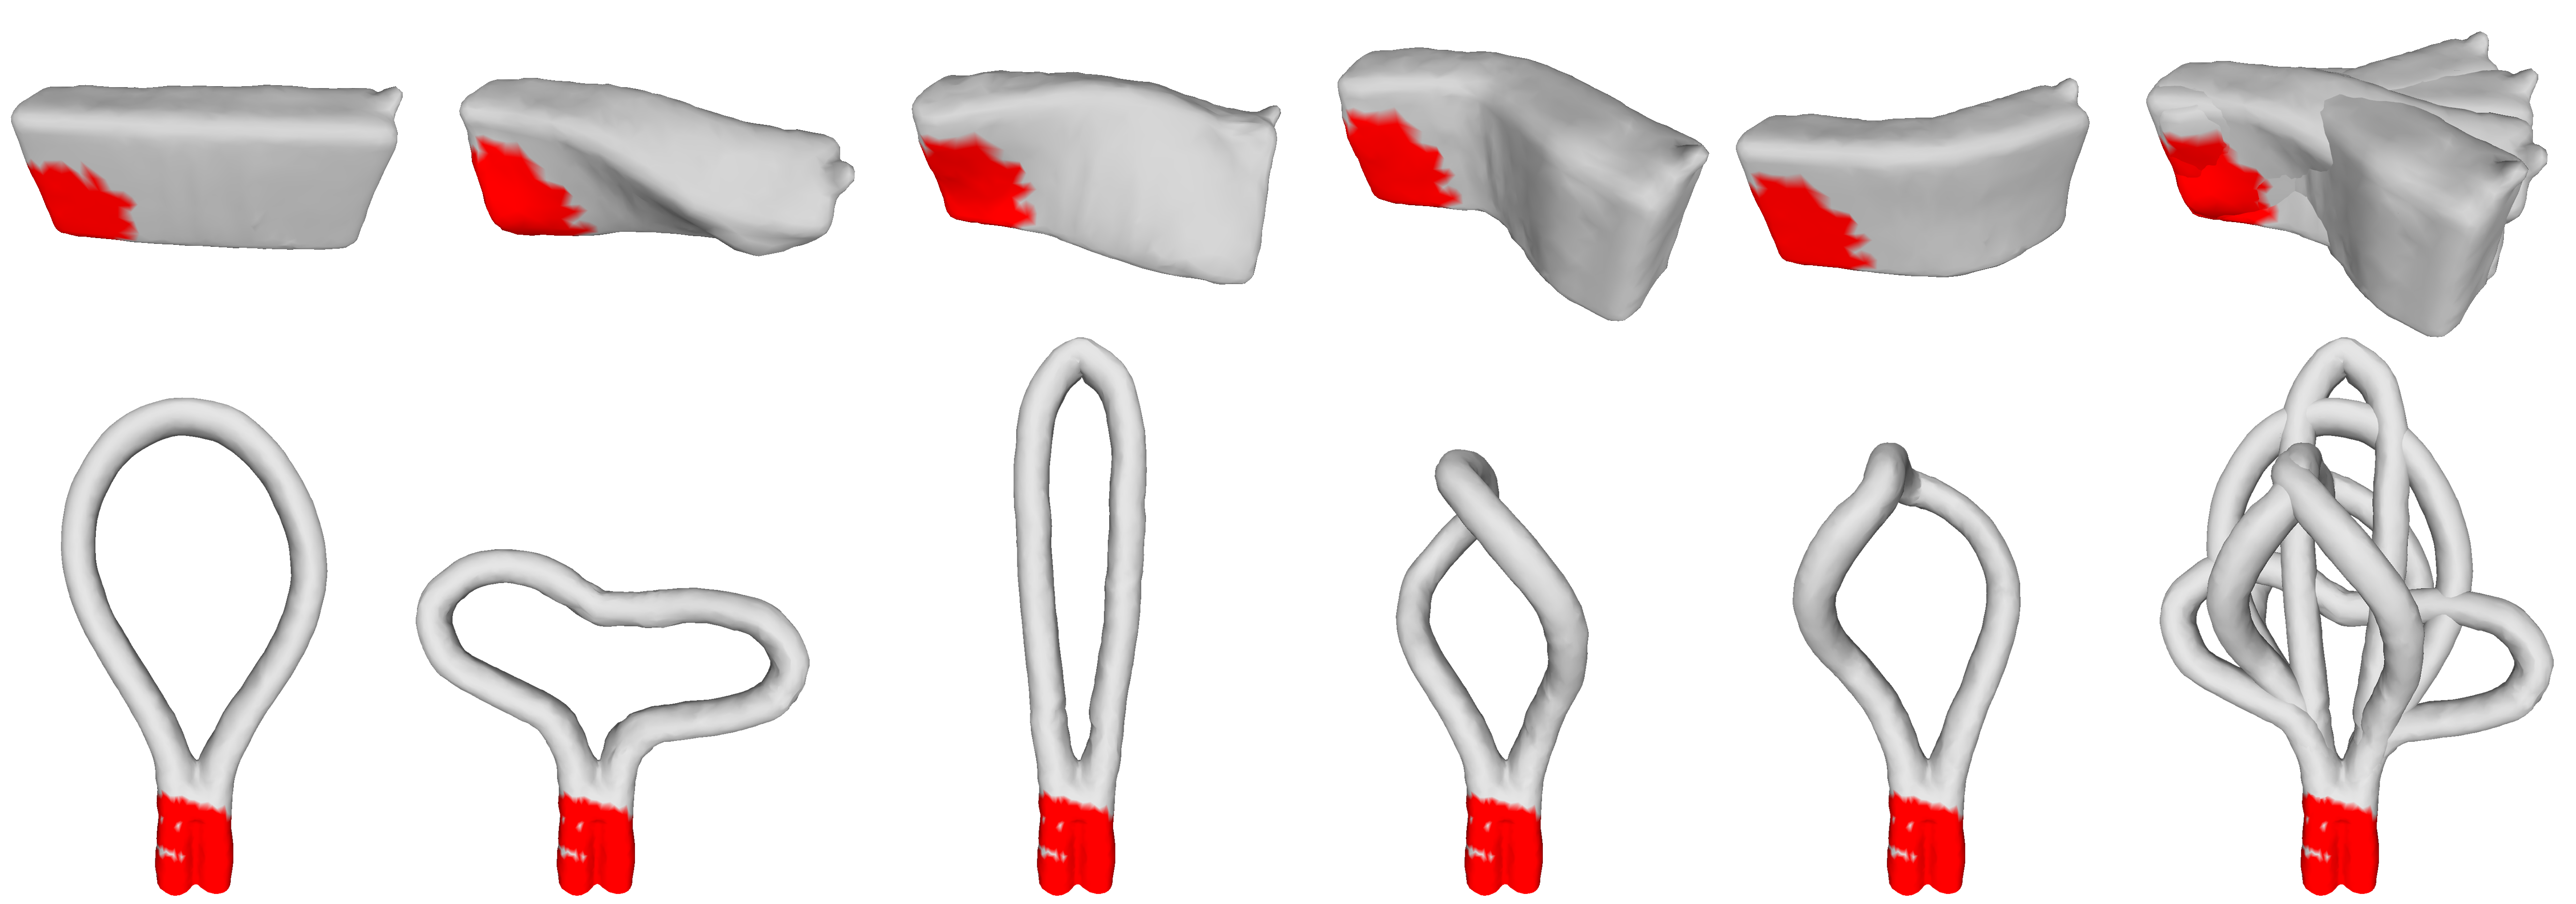
\includegraphics[width = \textwidth]{./Pictures/pillow_tube_keyframe.png}
    \caption{提取出的形变关键帧}
    \label{pillow_tube_keyframe}
\end{figure}

\section{形变子空间形变结果}\label{sec_subspace_res}
本文从形变图关键帧中提取特征向量,
特征向量描述的是形变模型相对初始模型的相对形变,
它由每个面片的形变形变梯度,即仿射变换中的非平移部分组成。
当对特征向量做插值并不是直接插值顶点的位置,
而是插值面片的变换。
所以本文中的特征向量插值不仅可以内插($0 \leq w \leq 1$),
在外插($w<0$或$w>1$)时依然能得到较好的结果。
图\ref{extrapolation}展示了各个样例上做内插和外插的结果。
图中的每一列分别为插值权重$w$的值分别为1.3、1、0.5、0、-0.5、-1、-1.3时的插值结果。
其中$w=0$时的模型为初始模型,
$w=1$时的模型为该特征向量对应的形变关键帧。
可以看出特征向量无论是内插还是外插,
甚至在权重为负数时仍然能得到自然的插值结果。
\begin{figure}[h]
    \centering
    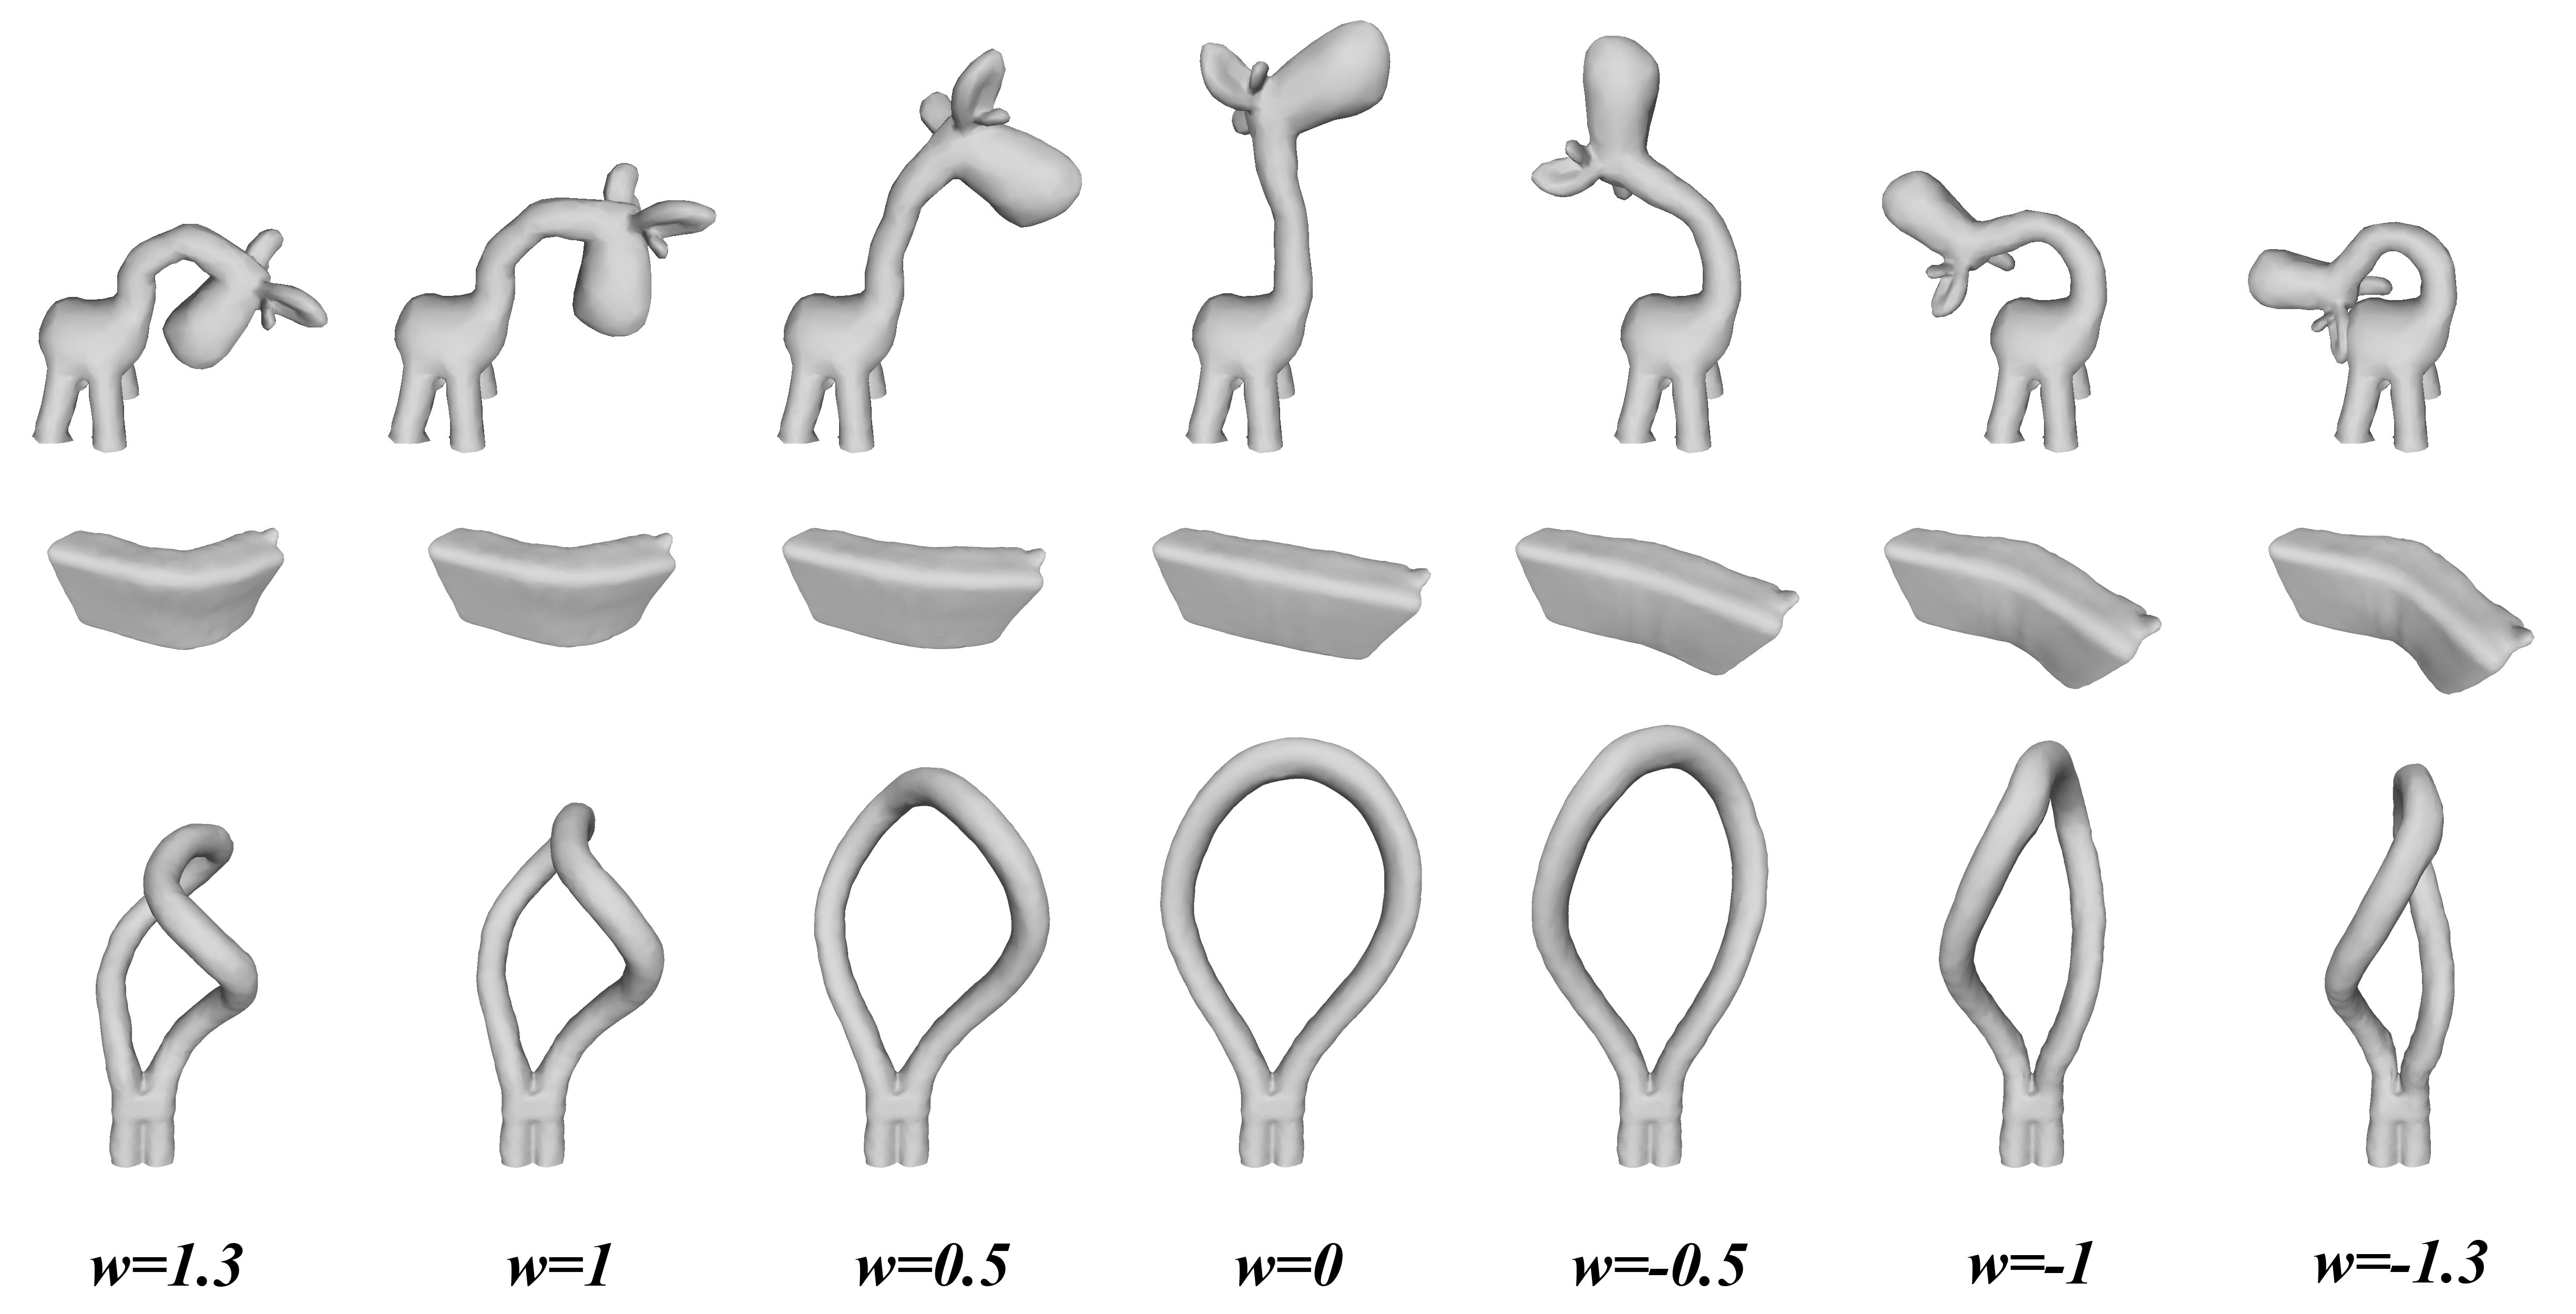
\includegraphics[width = \textwidth]{./Pictures/extrapolation.png}
    \caption{各模型上内插与外插的结果}
    \label{extrapolation}
\end{figure}

在基于形变子空间的模型修改方法里,
能量函数中的系数$\lambda_c$的值决定控制点的目标位置在形状修改时的权重。
当控制点仍然落在形变子空间内时,
$\lambda_c$的值对形变的结果并无明显的影响。
但当控制点被用户拖动到模型的形变子空间外的时候,
$\lambda_c$的值就决定了形状修改时的倾向。
图\ref{different_lambda}展示了$\lambda_c$取值不同时形状修改的结果。
图中位于模型头部的控制点被用户拖动到了形变空间之外的位置,
五张图从左至右分别为$\lambda_c$的值为1、10、50、100时形状修改的结果。
可以看出$\lambda_c$的值较小值,
形变修改的结果更倾向于让模型的形状落在模型的形变子空间内;
当$\lambda_c$的值较大的时候,
形变修改的结果更倾向于与让模型的形状更接近控制点。
图\ref{edit_result}展示了利用形变子空间形状修改得到的形变模型,
每幅图片下方的向量为各基向量的插值权重。
可以看出基于形变子空间的形状修改可以得到复杂而自然的形变结果。
\begin{figure}
    \centering
    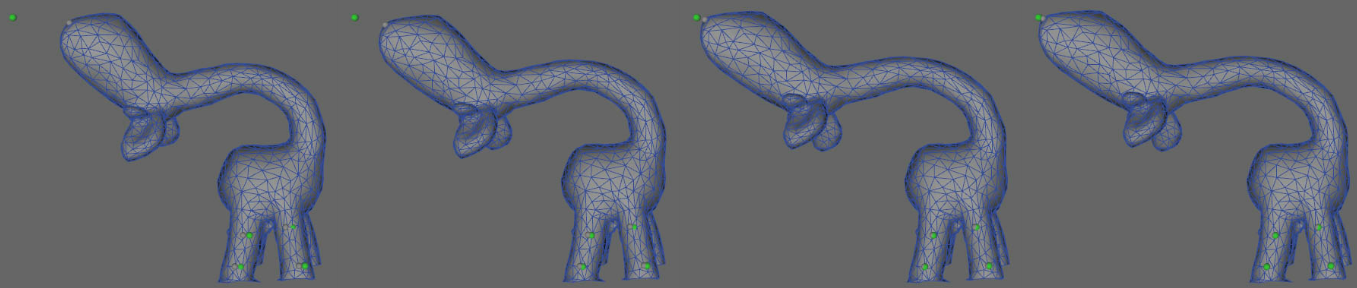
\includegraphics[width = 0.85\textwidth]{./Pictures/different_lambda.png}
    \caption{$\lambda_c=1/10/50/100$时形状修改的结果}
    \label{different_lambda}
\end{figure}
\begin{figure}
    \centering
    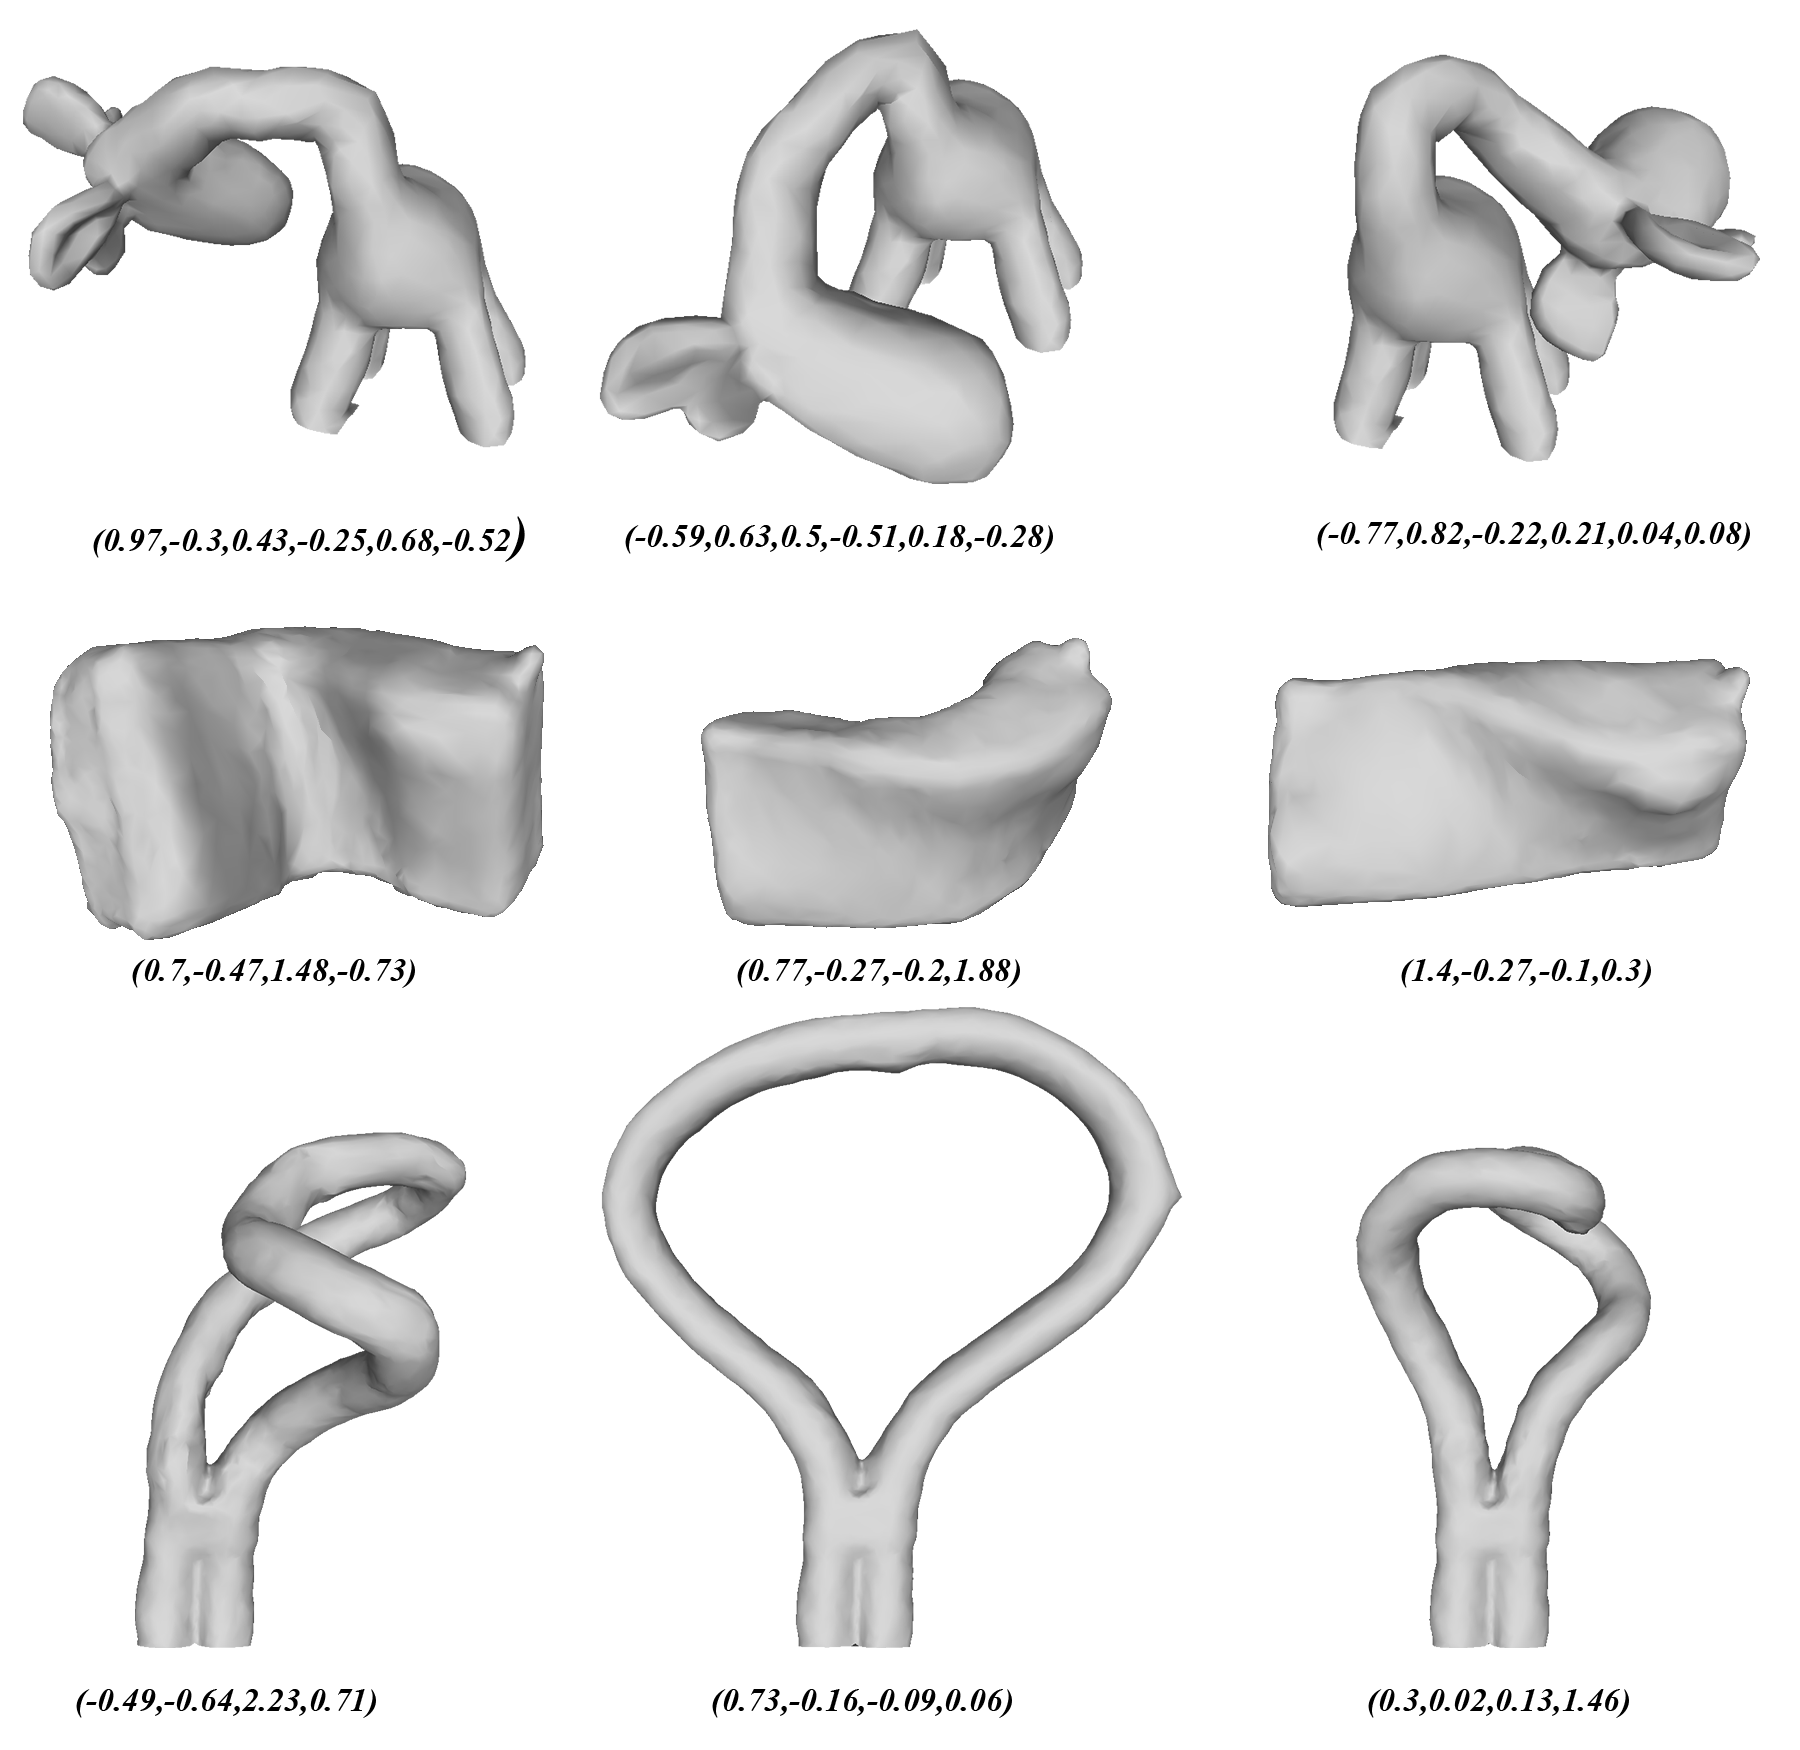
\includegraphics[width = 0.85\textwidth]{./Pictures/edit_result.png}
    \caption{通过模型修改得到的形变模型}
    \label{edit_result}
\end{figure}
\section{本章小结}
本章展示了分析了本文的实验结果。
首先,本章展示了在不同位姿下位姿估计算法的结果,以及位姿估计各阶段的耗时;
然后,本章展示了更多提取形变关键帧的结果;
最后,本章展示了特征向量的插值效果以及形变子空间形状修改的结果。